\section{Datos generales}
    \label{datos-generales} 
    Se considerará el caso idealizado de que infección ocurra con las en una comunidad aislada donde cada huésped definitivo (en este caso, un ser humano) tiene igual exposición de riesgo de infectarse y no está sujeto a procesos de nacimiento, muerte, inmigración o emigración.\\
    \begin{figure}
        \centering
         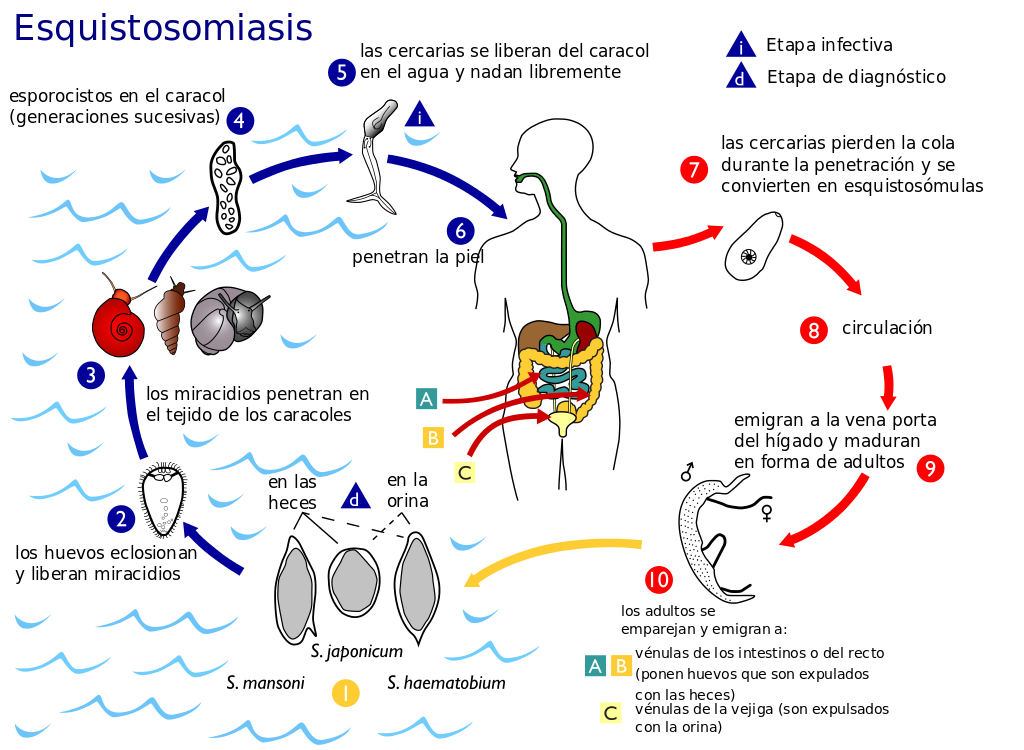
\includegraphics[scale=0.25]{Cap5-AnálisisEsquitosoma/img/ciclo_vital.png}
        \caption{Ciclo vital de un esquitosoma que infecta a un ser humano.}
    \end{figure}
    Cada huésped intermedio (en este caso, caracoles pulmonados acuáticos pertenecientes al género Lymnaea) tampoco está sujeto a procesos de inmigración o emigración pero sí al de nacimiento o muerte, pero bajo una simplificada hipótesis de que en cada instante en el que un caracol muera, un caracol no infectado nazca.\\
    Denotaremos como $N_1$ al número total de huéspedes definitivos (ser humano) en la población a analizar y $N_2$ al número total de huéspedes intermedios (caracoles) en la población a analizar.\\
    Si a cada ser humano de la población los etiquetamos del $1$ al $N_1$, se analizará un experimento por cada huésped definitivo $k$, donde $k=1,2,\ldots,N_1$, el cual será el mismo para cada poblador.
    Para cada $t\in[0,+\infty)$, introducimos las funciones,
    $$M_k(t)= \textit{Número de esquitosomas machos en el tiempo t, en el huésped k.}$$
    $$F_k(t)=\textit{Número de esquitosomas hembras en el tiempo t, en el huésped k.}$$
    Nociones de epidemiología nos dice que para que un huésped definitivo sea infectado depende de una pareja heterosexual de larvas de los esquistosomas (llamadas miracidios), por lo cual nuestro objetivo será registrar el número de parejas esquitosomas en un determinado huésped, en un tiempo $t$.\\Si asumimos que el encuentro entre cada miracidio hembra y macho es inevitable y cada larva es monógama, entonces de esto se puede deducir que el número de parejas de miracidios será nada más que el mínimo entre el número de miracidios machos y hembras.
    $$\gamma_k(t)=\min\{M_k(t),F(t)\}$$
    También es plausible postular que $M_k(t)$ y $F_k(t)$ para cada $t$ son variables aleatorias.\\
    Aunque es posible que un huésped intermedio sea penetrado por más de un miracidio, se cree que las infecciones múltiples no son importantes.
    
    % (\cite{JordanyWebbe}).
    En consecuencia, consideramos la unidad de infectividad en el huésped intermedio población como el huésped molusco individual, en lugar de la cantidad de parásitos que alberga y realizar un seguimiento de la infección en esta población mediante una función.\\
    Por ello, es necesario considerar cuál es la cantidad de huéspedes intermedios infectados (un caracol es llamado infectado si alberga al menos un miracidio), para ello será necesario definir $$S(t)= \textit{Número de caracoles infectados en el tiempo $t$.}$$
\begin{Obs}
   Para cada $t\geq 0$, $k=1,2,\ldots N_1$, es plausible postular que $M_k(t)$, $F_k(t)$, $S(t)$ son consideradas variables aleatorias y consecuentemente, las colecciones $\{M_k(t)\}_{t\geq 0}$, $\{F_k(t)\}_{t\geq 0}$ y $\{S(t)\}_{t\geq 0}$, procesos estocásticos.
\end{Obs}
Para determinar las distribuciones de probabilidad de las variables aleatorias de interés, es necesario hacer suposiciones adicionales.
Para este análisis se utilizará la definición infinitesimal del proceso particular de Poisson de nacimiento y muerte.\\ \\ 
% \begin{itemize}
%\item
 \textbf{Miracidios en el huésped definitivo.}\\
Para cada persona $k=1,2,\ldots,N_1, j=0,\thinspace 1,\thinspace\ldots$ será necesario conocer sus respectivas distribuciones iniciales $$q_j^{(k)}=P(M_k(0)=j)$$ $$p_j^{(k)}=P(F_k(0)=j)$$ para que el proceso pueda iniciar.\\
    Además para simplificar notación y cálculos, los procesos $M_k$ y $F_k$ tendrán la misma probabilidad de transición, es decir que será indiferente el que  cada parásito sea hembra o macho.
    Denotemos a la probabilidad de transición del estado $i$ al estado $j$ de un tiempo $s$ a un tiempo $t$ de $\{M_k(t)\}_{t\geq 0}$ y $\{F_k(t)\}_{t\geq 0}$ como $P_{i,j}(s,t)$, entonces, 
    $$P_{m,n}(s,t)=P\big(M_k(t)=n\thinspace|\thinspace M_k(s)=m\big)=P\big(F_k(t)=n\thinspace|\thinspace F_k(s)=m\big)$$
    $$k=1,2,\ldots,N_1, m,n\in\Z^+,0\leq s<t$$
    Por ello, aunque en los siguientes postulados se trata el caso de las cercarias macho, también aplica para las cercarias hembra.\\
    Al establecer las hipótesis sobre la iniciación (nacimiento) y la terminación (muerte)  estableceremos el símbolo $o(h)$ para indicar cualquier cantidad que se desvanezca más rápidamente que el $h$ cuando $h\rightarrow 0$ i.e. $\lim_{h\rightarrow 0}\frac{o(h)}{h}=0$\\
    A continuación pasamos a adaptar los postulados de un proceso de nacimiento y muerte para el análisis matemático de la cantidad de miracidios en un ser humano.
    \begin{enumerate}
        \begin{figure}
          \label{cuerpo1}
            \centering
             
\includegraphics[scale=0.075]{Cap5-AnálisisEsquitosoma/img/cuerpo-1.png}
            \caption{En un cuerpo se encuentran $m$ miracidios y muere uno.}
        \end{figure}
        \item Si $\mu_1>0$ es la razón de muerte instantánea de un esquistosoma.\\
        Para analizar la probabilidad de muerte de un estado arbitrario $m\in \N$ (que vendría a ser la cantidad de parásitos en un ser humano) al tiempo $t$, donde cada uno tiene la misma media de probabilidad $\mu_1$ de morir y por lo tanto cada uno también tiene la misma probabilidad de muerte $P_{1,0}(t, t+h)=\mu_1 h + o(h)$, entonces, 
        $$P_{m ,m-1}(t,t+h)=mP_{1,0}(t,t+h)=\mu_1 mh+o(h)$$
         \item  Sea $\nu_{11}$ la tasa de liberación instantánea de cercarias por caracol infectado (factor biológico) y $\nu_{12}$ la probabilidad de que una cercaria liberada infecte a un ser humano (factor ambiental).\\
         \begin{figure}
         \label{cuerpo2}
            \centering
             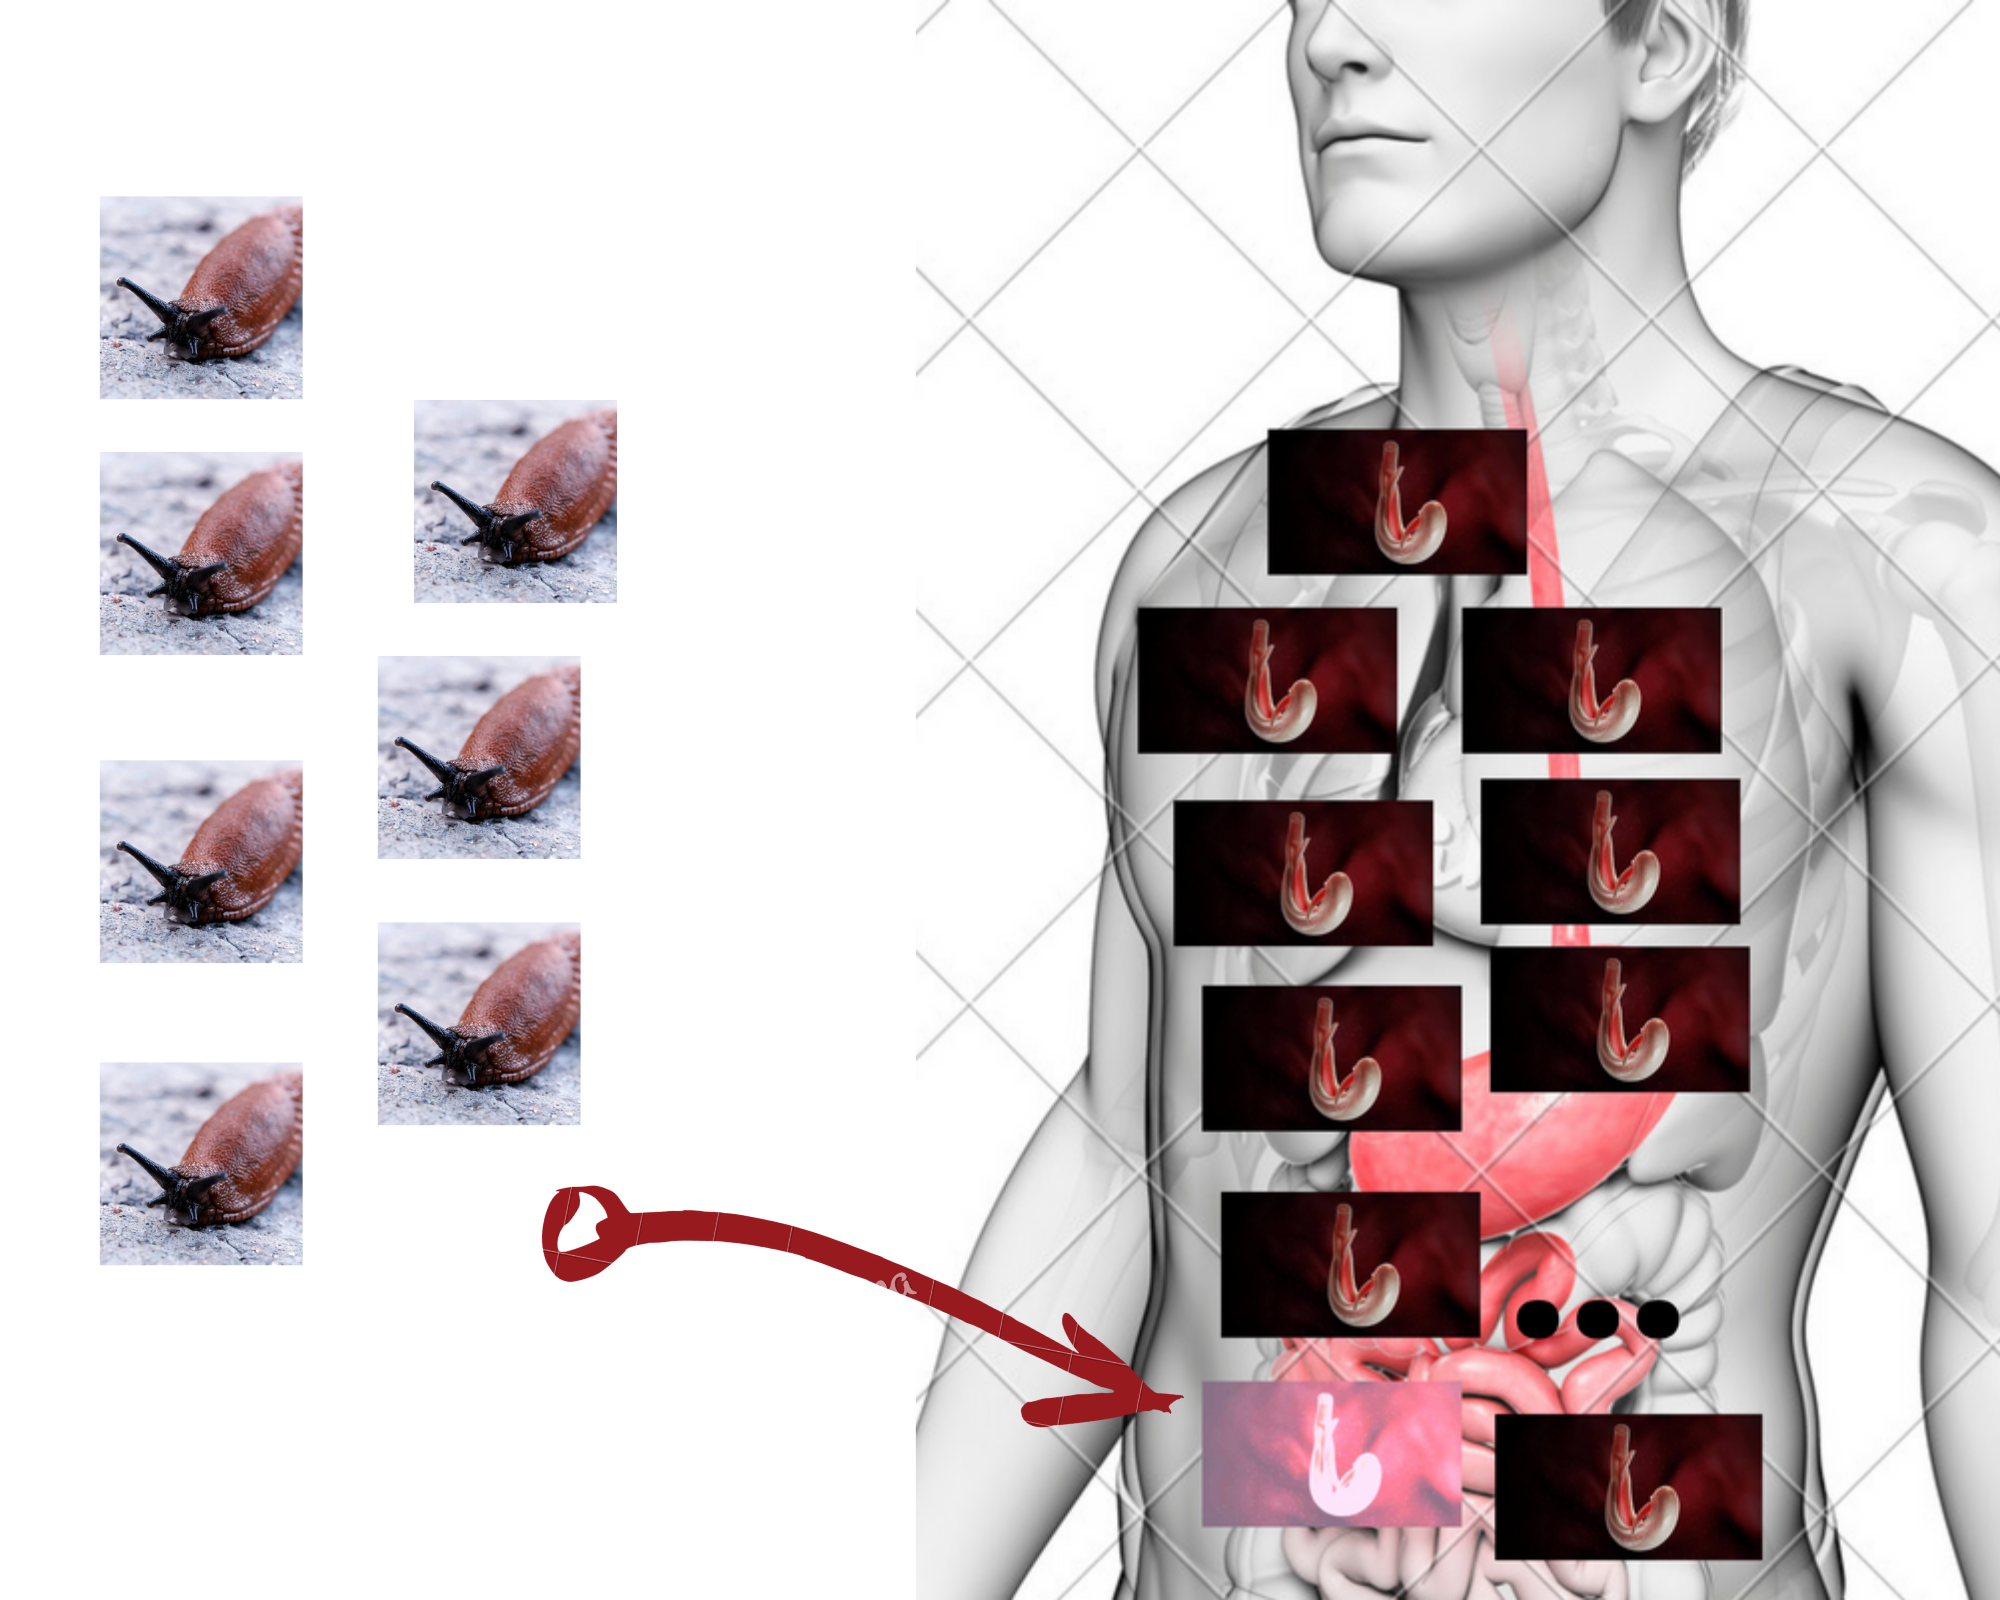
\includegraphics[scale=0.075]{Cap5-AnálisisEsquitosoma/img/cuerpo-2.png}
            \caption{En un cuerpo se encuentran $m$ miracidios y muere uno.}
        \end{figure}
        Denotemos $\nu_1=\nu_{11}\cdot\nu_{12}$, que vendría a ser la razón de parásitos que infectan a un ser humano y por ende, cada parásito tiene la misma probabilidad de infectar a un ser humano de $P_{0,1}(t, t+h)=\nu_1 h + o(h).$ Por lo tanto, para $m\in\N$ , $h\rightarrow 0$, la probabilidad de que un nuevo parásito infecte a un ser humano (ya sea macho o hembra) estaría dado por  $2P_{m,m+1}(t,t+h)=S(t)P_{0,1}(t, t+h)=\nu_1S(t)h+o(h)$.\\Si reemplazamos el valor de $S(t)$ por el de su esperanza $E[S(t)]$, se tiene,
        $$P_{m,m+1}(t,t+h)=\frac{1}{2}\nu_1E[S(t)]h+o(h)$$
        \item Aunque es posible para un huésped ser infectado por más de un miracidio al mismo tiempo o que al mismo tiempo mueran más de dos de estos parásitos, estos no generan cambios plausibles, por lo cual la probabilidad de más de un salto será $o(h)$. Es por eso que las transiciones de un estado $j$ solo son posibles a los estados $j+1$ o $j-1$ en un intervalo corto de tiempo (casi instantáneo), es decir, en un intervalo $[t,t+h)$, donde $h\rightarrow 0$.
        $$P_{m,m+n}(t,t+h)=o(h), n>1$$
        \item Al tiempo $t$, hay $n$ parásitos y no ocurre ningún cambio en el intervalo $[t,t+h)$.
         $$P_{m,n}(t,t+h)= 1-\frac{1}{2}\nu_1E[S(t)]hP_n(t)-\mu_1 P_{n}(t)h+o(h)$$
    \end{enumerate}
\begin{comment}
    \item \textbf{Miracidios en el huésped intermedio}\\
    Sea $\Pi$ la medida de probabilidad de $\{S(t)\}_{t\leq 0}$.
    Denotemos $\Pi_{i,j}(s,t)$ a la probabilidad de cambio de $i$ a $j$ caracoles infectados durante el intervalo de tiempo $[s,t)$, $$\Pi_{i,j}(s,t)=\Pi(S(t)=j|\thinspace S(s)=i)$$ $$i,j=1,2,\ldots,N_2,0\leq s<t$$ con distribución inicial, $$\pi_i=\Pi(S(0)=i)\quad \quad i=1,2,\ldots,N_2$$
    Pasamos a adaptar los postulados de un proceso de nacimiento y muerte para el análisis matemático de la cantidad de caracoles infectados.
    \begin{enumerate}
        \item  Se consideran que $j$ solo es posible al estado $j+1$ o $j-1$ en un intervalo corto de tiempo entre $t$ y $t+h$, mientras que la probabilidad de que suceda más de una infección en el intervalo instantáneo de tiempo $[t,t+h)$ es $o(h)\rightarrow 0$.
        \item Sea $\mu_2>0$ la razón de muerte instantánea de un caracol infectado, entonces la probabilidad que un caracol infectado muera está dado por, $\Pi_{10}(t,t+h)=\mu_2 h+ o(h)$. La probabilidad de cambio de $i$ a $i+1$ caracoles está dado por, $$\Pi_{i,i-1}(t,t+h)=i\Pi_{10}(t,t+h)=\mu_2 i h+o(h)\quad i\geq1,h\rightarrow 0$$
        \item Sea $\nu_{21}$ la tasa de colocación instantánea de una esquistosoma hembra apareada (factor biológico), $\nu_{22}$ es la probabilidad de que un huevo fertilizado de origen a un miracidio que infecte a un caracol no infectado (factor ambiental que depende principalmente de las condiciones sanitarias e higiénicas).\\
        Si $\nu_2=\nu_{21}\cdot\nu_{22}$ es el valor esperado instantáneo de caracoles infectados. La cantidad de parejas de esquitosomas en el tiempo $t$ por cada habitante $k=1,2,\ldots N_1$ es $\gamma_k(t)$, por lo tanto la cantidad total de esquitosomas en toda la población al tiempo $t$ sería $\sum_{k=1}^{N_1}\gamma_k(t)$ y por eso se obtiene que $\Pi_{01}(t,t+h)=\nu_2 \big(\sum_{k=1}^{N_1}\gamma_k(t)\big)h+o(h)$.\\
        Si reemplazamos el valor de $\sum_{k=1}^{N_1}\gamma_k(t)$ por su esperanza que $E\big[\sum_{k=1}^{N_1}\gamma_k(t)\big]$ se obtiene que
        $$\Pi_{i,i+1}(t,t+h)=(N_2-i)P_{0,1}(t,t+h)= \nu_2(N_2-i)E\bigg[\sum_{k=1}^{N_1}\gamma_k(t)\bigg]h+o(h)\quad ,i\leq N_2-1, h\rightarrow 0$$
        \item La probabilidad de que no haya ningún cambio entre el tiempo $t$ y $t+h$ se reduciría a  $\Pi_{i,i}(t+h)=1-\Pi_{i,i-1}(t,t+h)-\Pi_{i,i+1}(t,t+h)$, esto es $$\Pi_{i,i}(t,t+h)=1-\mu_2 i h-\nu_2(N_2-i)E\bigg[\sum_{k=1}^{N_1}\gamma_k(t)\bigg]h+o(h)$$
    \end{enumerate}
\end{itemize}
    \begin{Prop}
    \begin{eqnarray}
        E[S(t)]=\sum_{j=1}^{N_2}j\sum_{i=1}^{N_2}\pi_{i}\Pi_{i,j}(0,t).
        \label{equation-E(S)-probInicial}
    \end{eqnarray}
\end{Prop}
\begin{Prop}
    \begin{eqnarray}
    \label{equation-E(gamma)-probInicial}
        \begin{array}{cr}
            E\bigg[\sum_{k=1}^{N_1}\gamma_k(t)\bigg]=& \sum_{k=1}^{N_1}\sum_{r=1}^\infty\bigg[\sum_{\rho=0}^\infty p_\rho^{(k)}P_{\rho,r}(0,t)\sum_{n=r}^\infty\sum_{m=0}q_m^{(k)}P_{m,n}(0,t) \\
             &+\sum_{n=r+1}^\infty\sum_{\rho=0}^\infty p_j^{(k)}P_{\rho, n}(0,t)\sum_{m=0}^\infty q_m^{(k)}P_{m,r}(0,t)\bigg]
        \end{array}
    \end{eqnarray}
\end{Prop}
Usando las relaciones \ref{equation-E(S)-probInicial} y \ref{equation-E(gamma)-probInicial} los precedentes postulados pueden ser expresados usando solo las distribuciones iniciales y las transiciones $\Pi_{i,j}(0,t)$ y $P_{m,n}(0,t)$.\\
\end{comment}
%%%%%%%%%%%%%%%%%%%%%%%%%%%%%%%%